\experiment{Toma de Datos Experimentales}

Para la adquisición de datos, se ensambló completamente el sistema de
tres péndulos físicos acoplados. Se instaló un sensor rotacional
\emph{Cassy} en el soporte de cada péndulo, alineado coaxialmente con su
eje de giro. Esta disposición, visible en la \cref{fig:set-up},
permitió registrar el desplazamiento angular \(\theta_i(t)\) de cada
barra de forma independiente. Los resortes de acoplamiento se fijaron
a las barras según las especificaciones del diseño experimental,
estableciendo así la interacción mecánica entre los péndulos.

Una vez configurado el montaje, se realizaron mediciones para cinco
distintas configuraciones de acoplamiento del sistema. Estas
configuraciones, que varían los puntos de anclaje de los resortes
entre los péndulos, se ilustran esquemáticamente en la
\cref{fig:configs}, junto con la codificación utilizada para
identificarlas. Para cada una de estas cinco configuraciones,
el sistema se observó bajo tres condiciones de excitación inicial
(desplazamiento angular inicial):
\begin{itemize}
	\item Desplazamiento de un solo péndulo lateral (i.e. péndulo 1),
		codificado como (100).
	\item Desplazamiento del péndulo central (péndulo 2), codificado
		como (010).
	\item Desplazamiento simultáneo y simétrico (o antisimétrico,
		según el caso) de los dos péndulos laterales (péndulos 1 y 3),
		codificado como (101).
\end{itemize}
Los datos de la evolución temporal del ángulo de cada péndulo para
cada ensayo fueron registrados automáticamente por el sistema \emph{Cassy}
y almacenados digitalmente para su posterior análisis. Se procuró
que cada registro tuviera una duración aproximada de
\qty{30}{\second} para capturar múltiples oscilaciones.

\begin{figure}[htbp!]
	\centering
	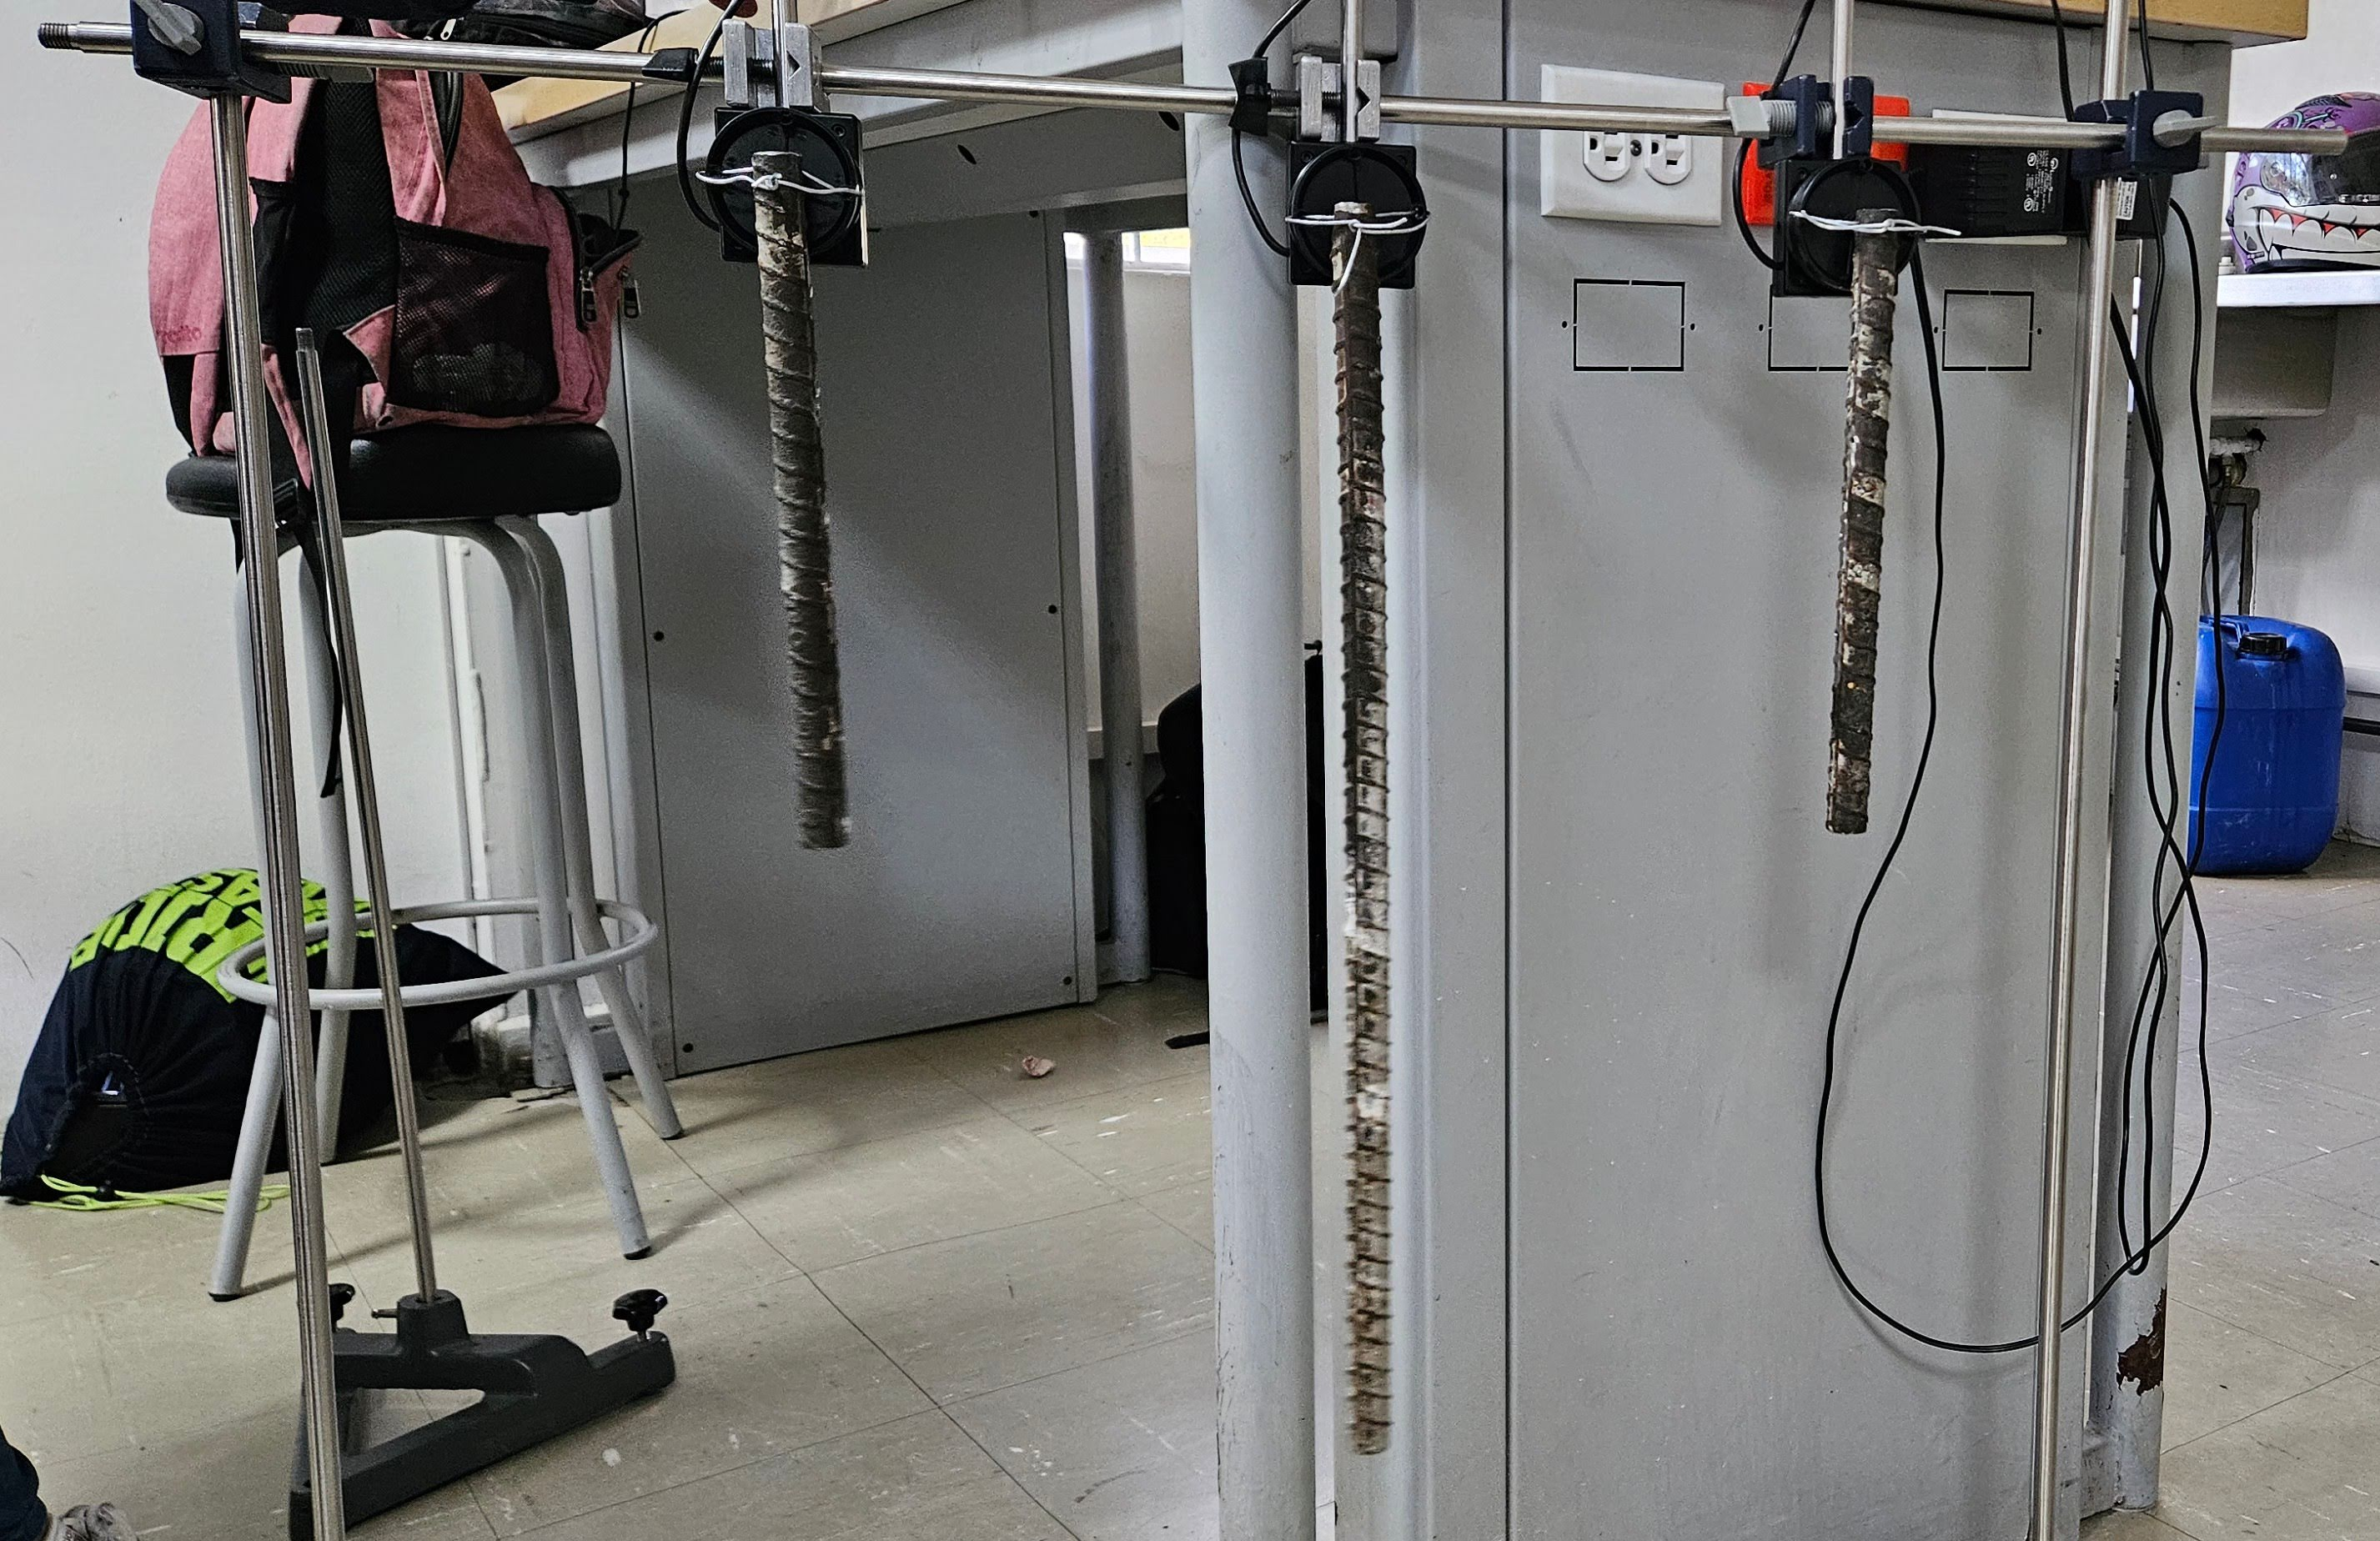
\includegraphics[width=0.6\linewidth]{./Figures/set-up.jpeg}
	\caption{Montaje experimental completo con los tres péndulos
		acoplados y los sensores rotacionales \emph{Cassy} posicionados para
	medir el ángulo de cada péndulo.}
	\label{fig:set-up}
\end{figure}

\begin{figure}[htbp!]
	\centering
	\begin{subfigure}[b]{0.3\textwidth}
		\centering
		\scalebox{-1}[1]{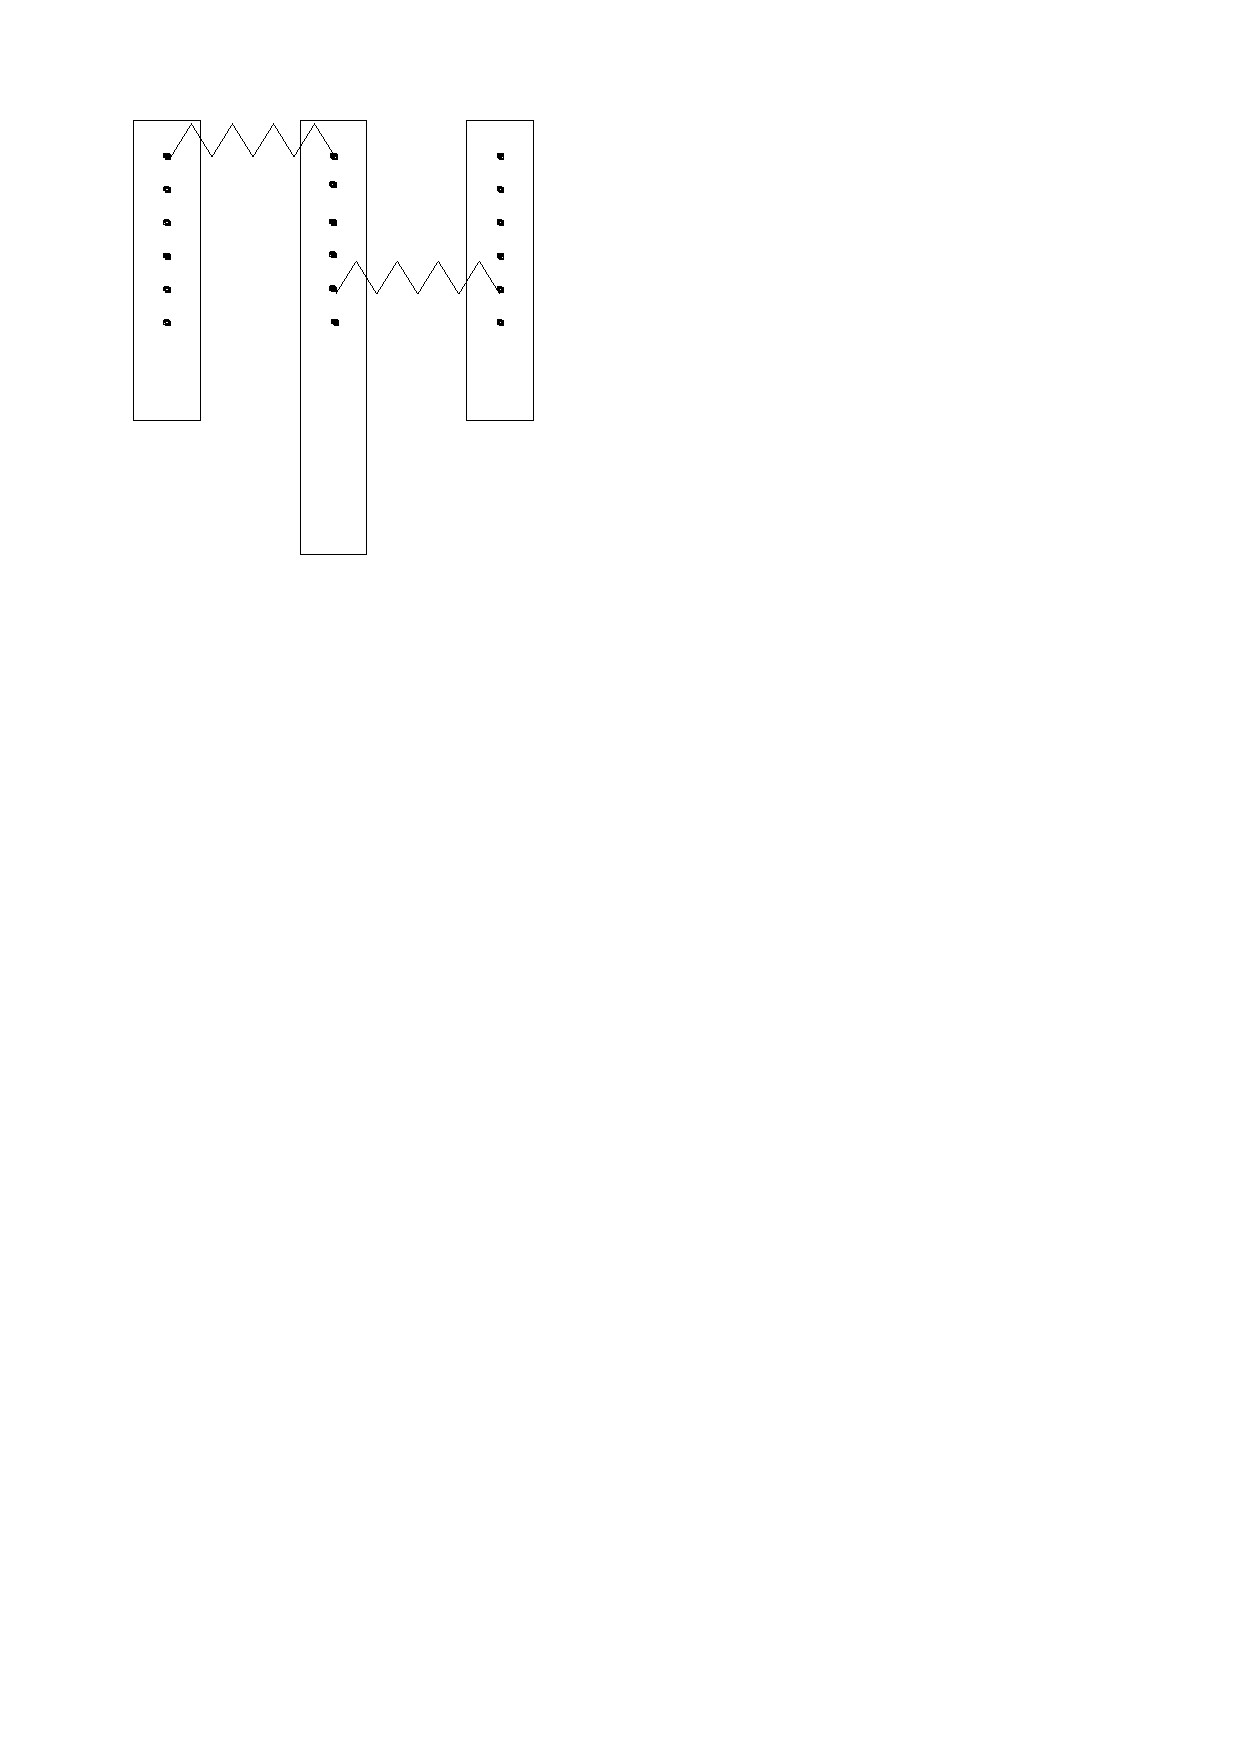
\includegraphics[width=\linewidth]{./Figures/15.pdf}}
		\caption{Configuración 5-1}
		\label{fig:conf-1-5}
	\end{subfigure}
	\hfill
	\begin{subfigure}[b]{0.3\textwidth}
		\centering
		\scalebox{-1}[1]{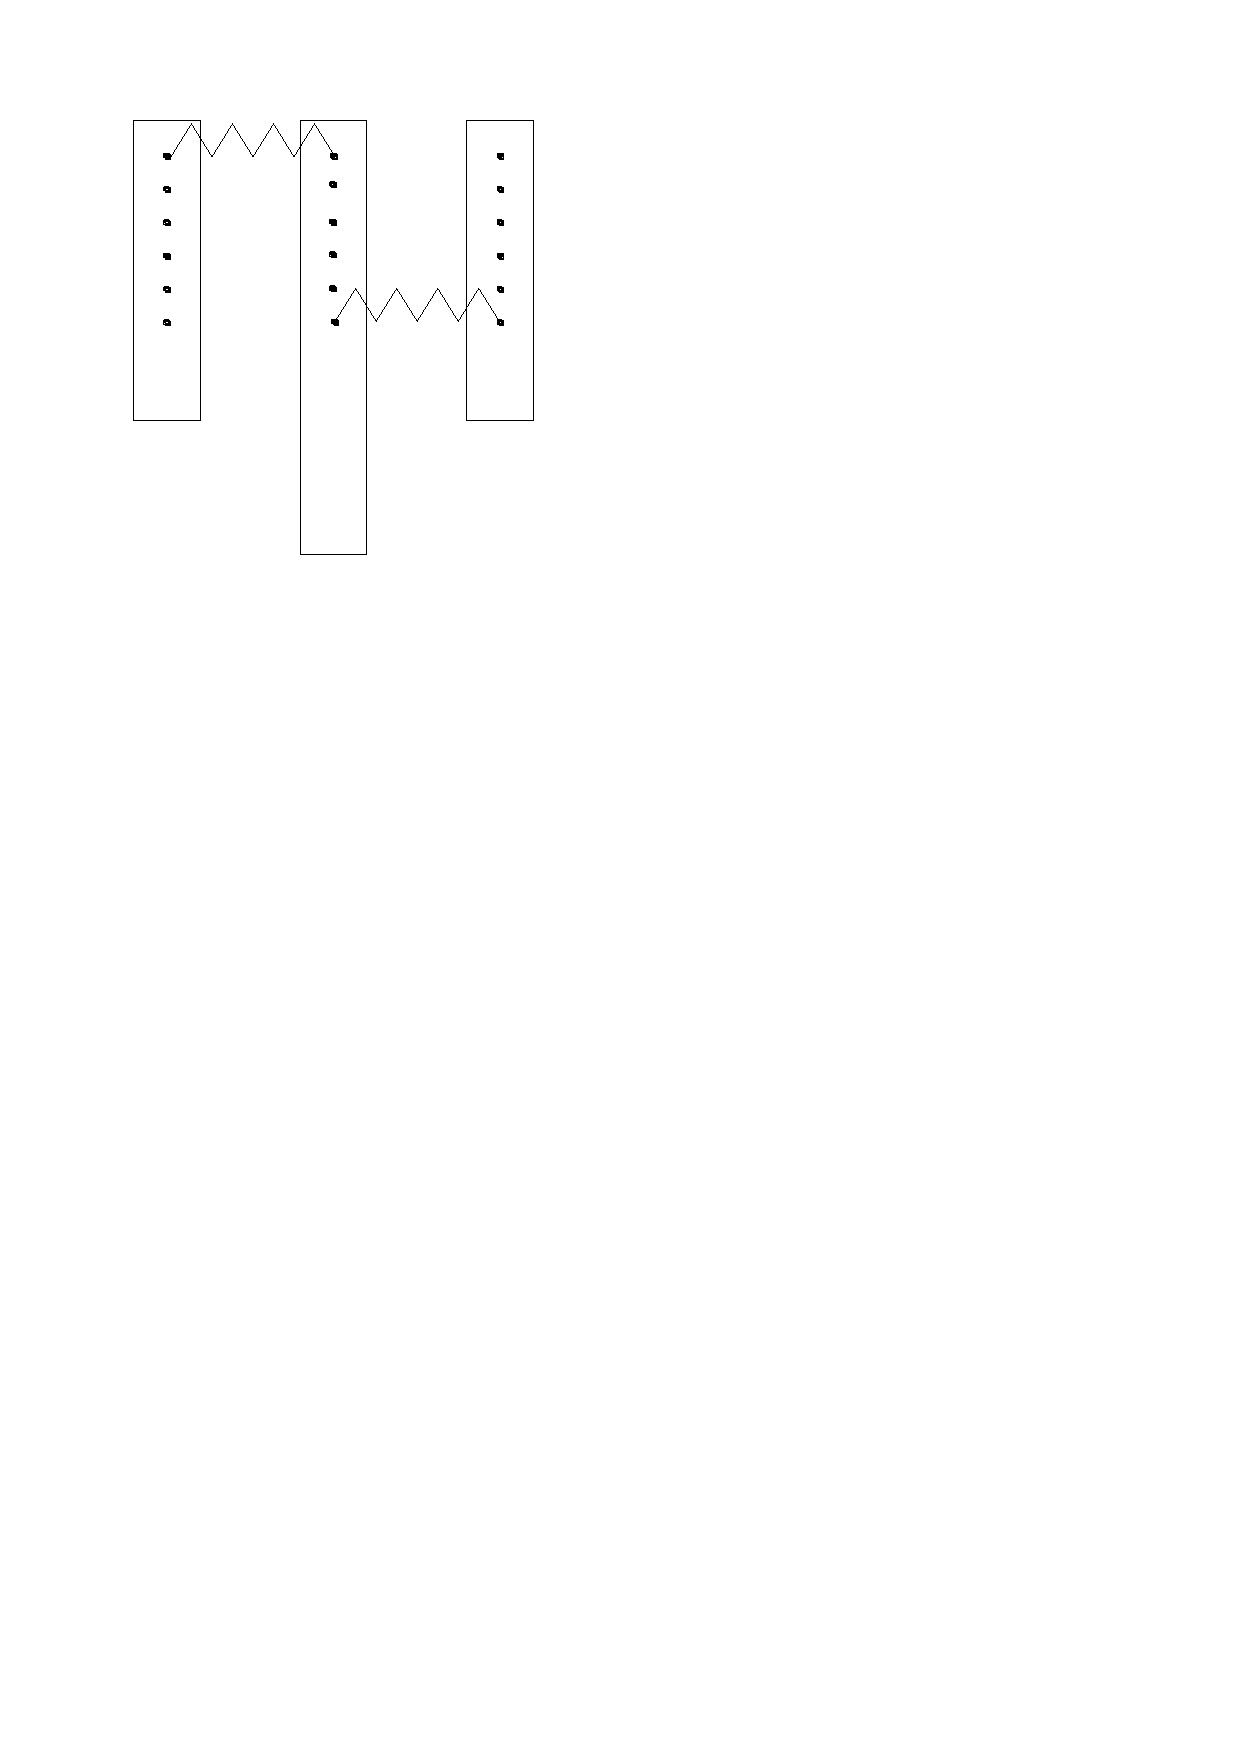
\includegraphics[width=\linewidth]{./Figures/16.pdf}}
		\caption{Configuración 6-1}
		\label{fig:conf-1-6}
	\end{subfigure}
	\hfill
	\begin{subfigure}[b]{0.3\textwidth}
		\centering
		\scalebox{-1}[1]{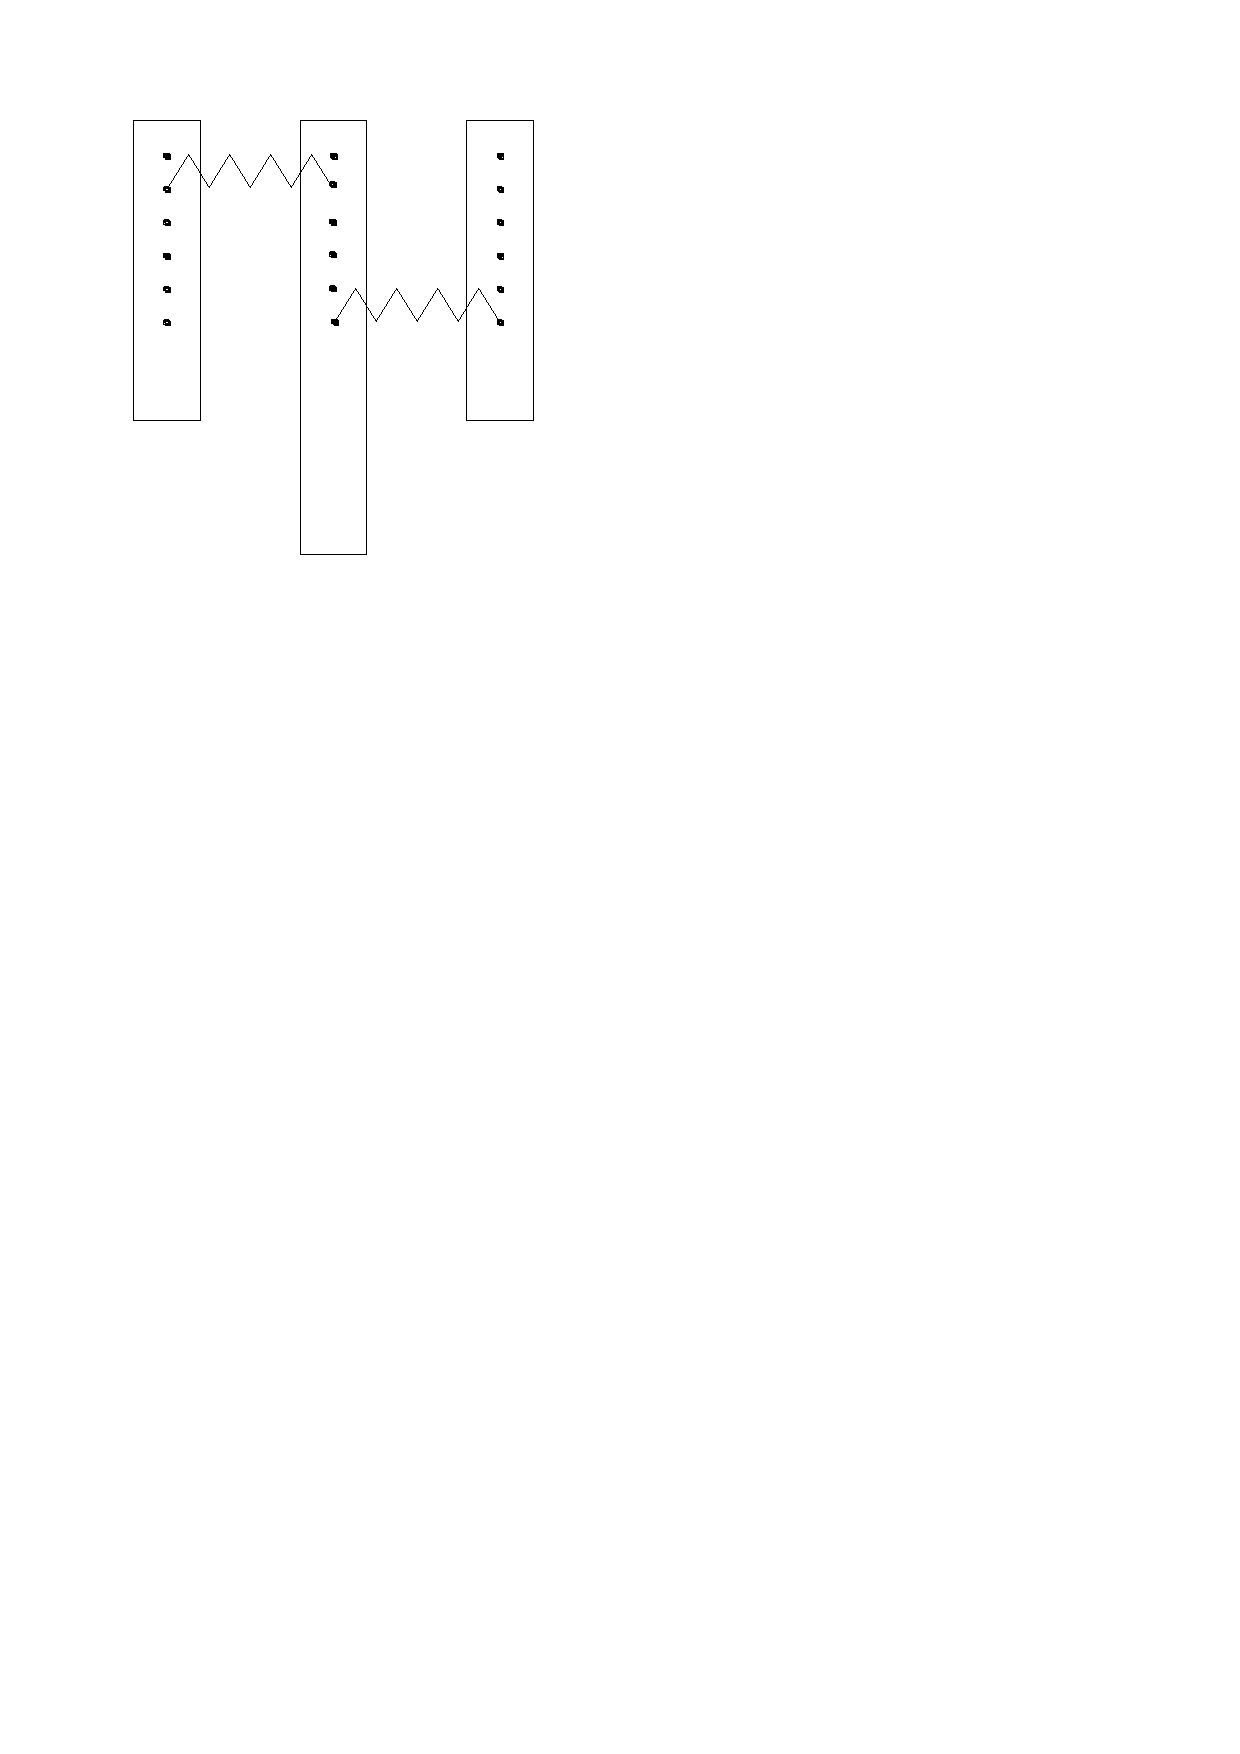
\includegraphics[width=\linewidth]{./Figures/26.pdf}}
		\caption{Configuración 6-2}
		\label{fig:conf-2-6}
	\end{subfigure}

	\vspace{0.5cm}

	\begin{subfigure}[b]{0.3\textwidth}
		\centering
		\scalebox{-1}[1]{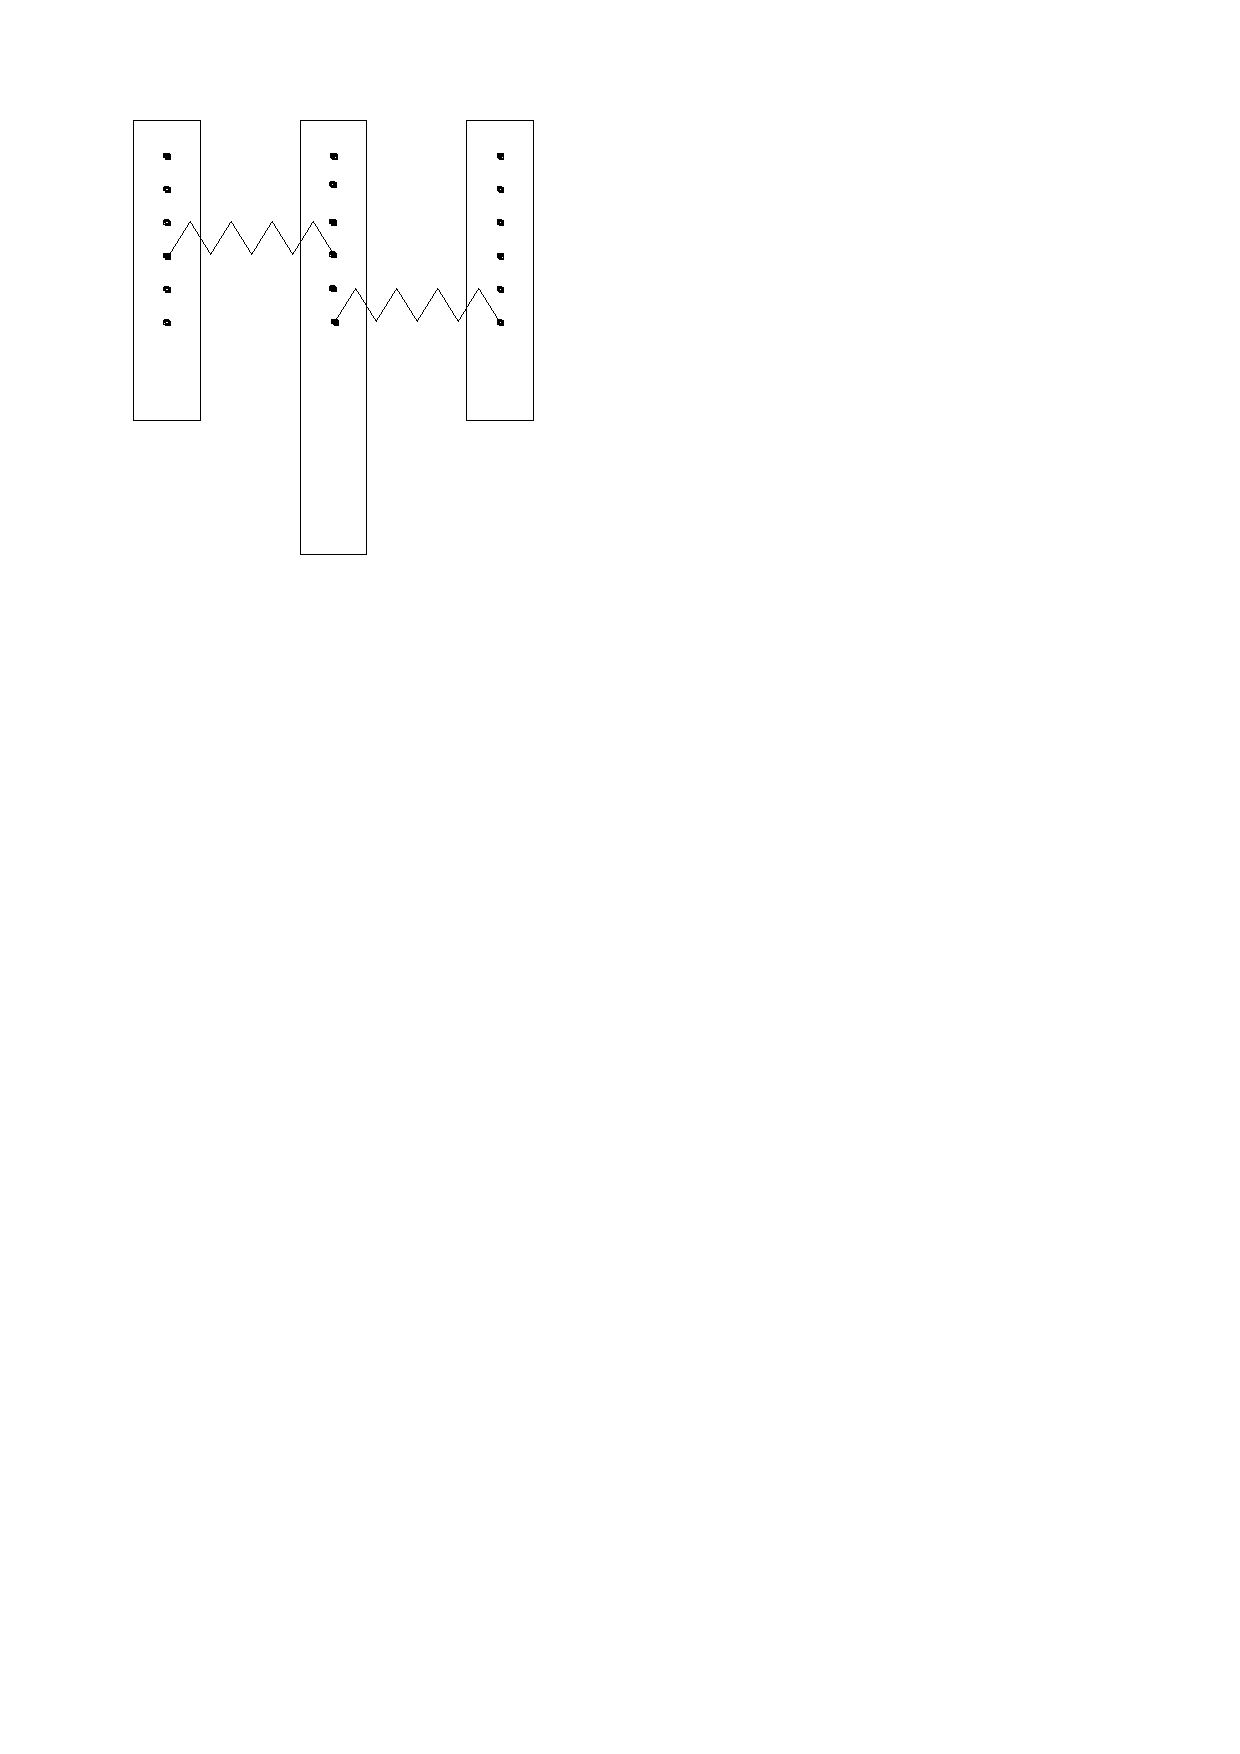
\includegraphics[width=\linewidth]{./Figures/46.pdf}}
		\caption{Configuración 6-4}
		\label{fig:conf-4-6}
	\end{subfigure}
	\hspace{0.1\textwidth}
	\begin{subfigure}[b]{0.3\textwidth}
		\centering
		\scalebox{-1}[1]{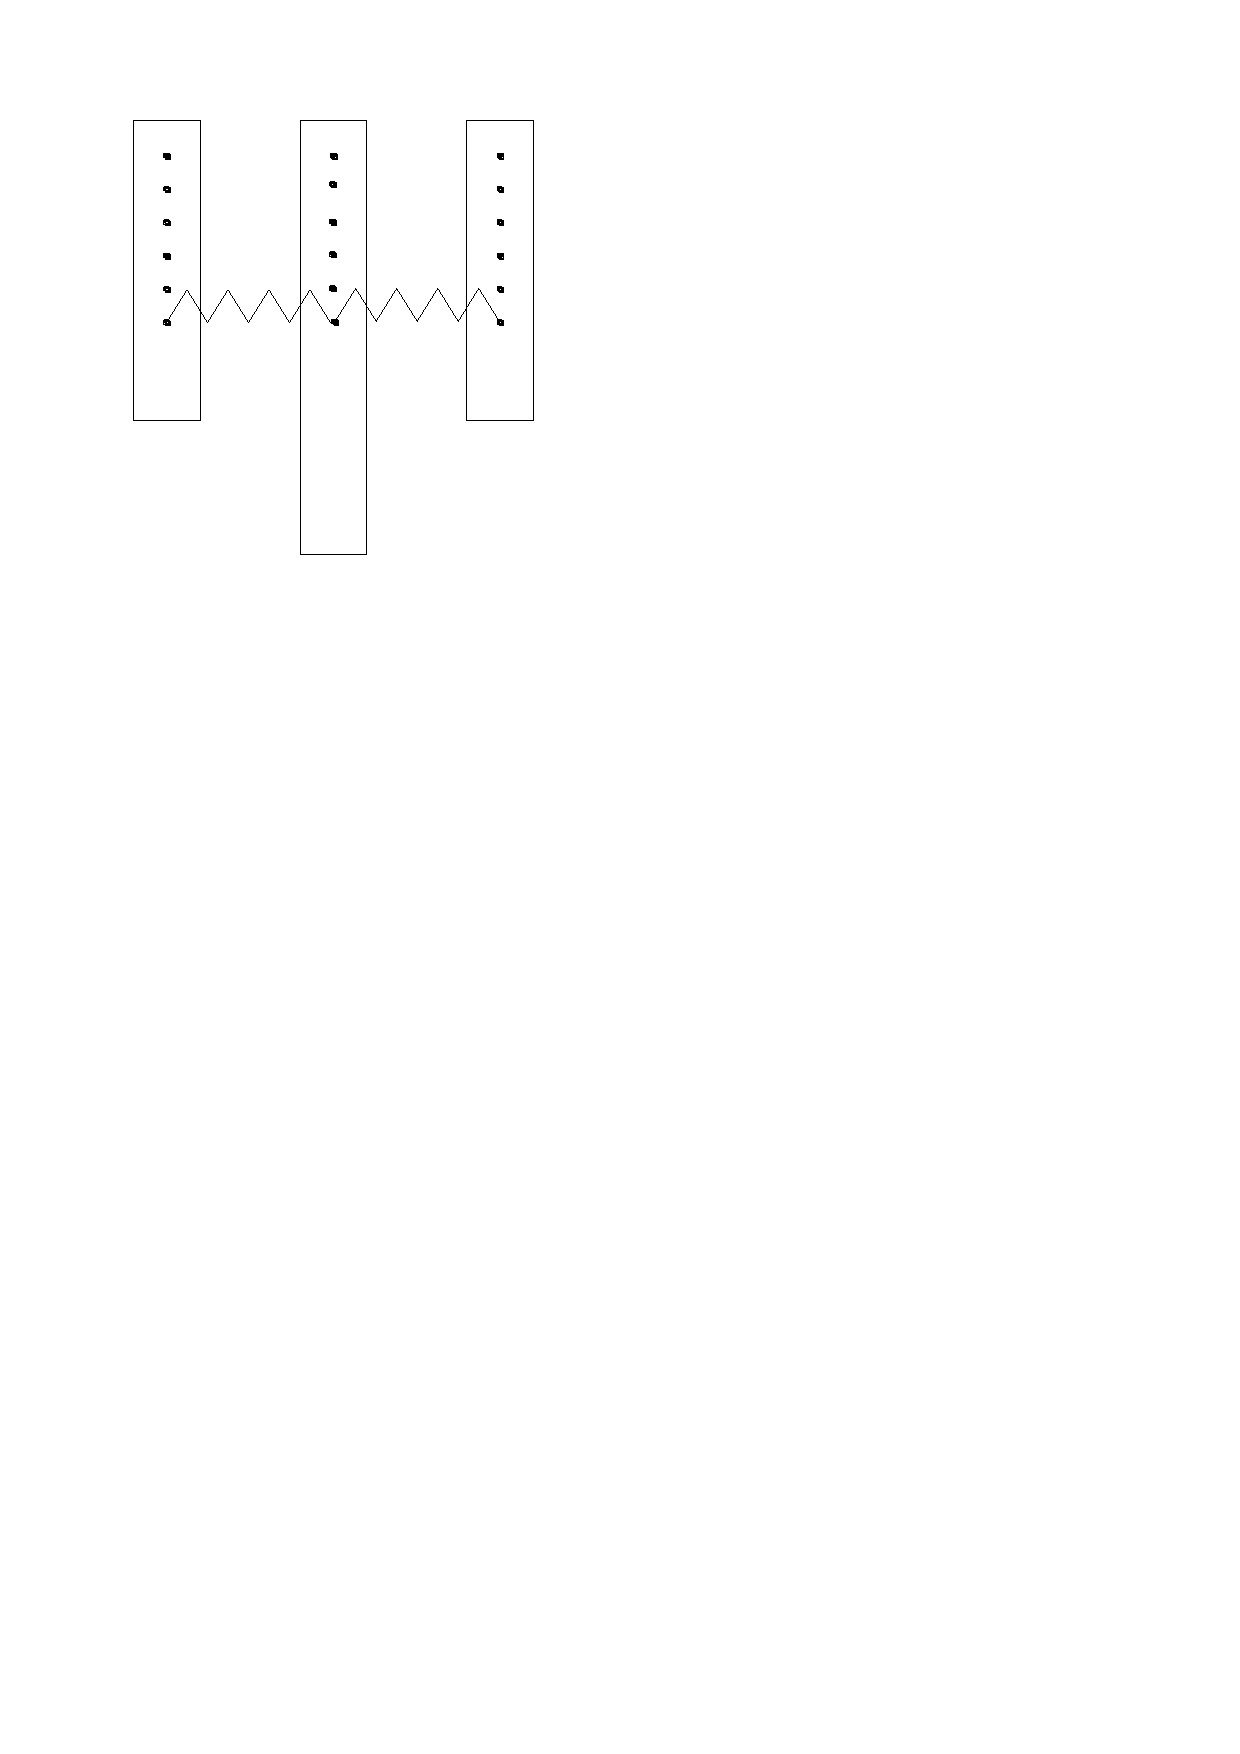
\includegraphics[width=\linewidth]{./Figures/66.pdf}}
		\caption{Configuración 6-6}
		\label{fig:conf-6-6}
	\end{subfigure}

	\caption{Representación esquemática de las cinco configuraciones de
		acoplamiento de resortes estudiadas. La nomenclatura 'X-Y' en cada
		subfigura (e.g. 5-1) denota los puntos de anclaje de los resortes
	en orificios específicos de los péndulos adyacentes.}
	\label{fig:configs}
\end{figure}
